\chapter{项目文件、排障与进阶}
\label{ch:projects}

\begin{introduction}
  \item 看懂 \texttt{.pieproj}：格式 17 的 JSON 结构与稳定枚举值；
  \item 了解自动保存、原子写入与“最近项目”的工作方式；
  \item 遇到故障时按“检查页 $\rightarrow$ 生成代码页 $\rightarrow$ 烧录页”
        的顺序定位；
  \item 知道 Web/Android 版能做什么、不能做什么，以及进阶的三条路。
\end{introduction}

本书各章都围绕项目文件工作：每填一个字段，PIE-Block 就把它写进一个
\texttt{.pieproj}。本章讲清这个文件的里里外外——格式、保存策略、版本
兼容——然后给出全书共用的排障路径与进阶方向。示例文件都在随书仓库
\texttt{book/examples/} 下，可以直接打开。

\section{.pieproj：格式 17 的 JSON}

\texttt{.pieproj} 是 UTF-8 编码的 JSON 文件。下面是随书示例
\texttt{infantry-standard.pieproj} 的骨架（数值有删节）：

\begin{lstlisting}[style=pieblockc,
  caption={\texttt{.pieproj} 格式 17 的结构（节选）},
  label={lst:ch10-pieproj}]
{
  "format_version": 17,
  "name": "教材示例：标准步兵",
  "project_kind": "infantry",
  "guide_progress": {
    "current_step_id": "remote",
    "visited_step_ids": ["remote"]
  },
  "config": {
    "remote": {"channel": 36, "deadzone": 100},
    "chassis": {"enabled": true, "left_front": {"pin": "P74 P24", "direction": "forward"}, "...": "..."},
    "feeder_pin": "P60",
    "yaw": [{"drive": "servo", "pin": "MP74", "direction": "forward", "mid_offset": 0}],
    "friction_mode": "brushlessEsc",
    "friction_p64_max_duty": 700,
    "friction_p66_max_duty": 800
  }
}
\end{lstlisting}

几个设计要点：

\begin{itemize}
  \item \textbf{稳定枚举值}：\texttt{project\_kind} 保存
        \texttt{infantry/engineer/debug/music}，步骤 ID 保存
        \texttt{remote/pwm/strategy/mappings/review/code/deploy} 等英文
        稳定值——界面文案怎么改，文件都保持机器可读；
  \item \textbf{进度也是数据}：\texttt{guide\_progress} 记住离开时所在的
        步骤与访问范围，重开项目接着上次继续；
  \item \textbf{派生物不入文件}：生成的 C 代码、HEX、编译日志、编译器
        选择都不写进 \texttt{.pieproj}——配置是唯一的真相源，产物随时
        可以从配置重新推导；
  \item \textbf{格式版本隔离}：\texttt{format\_version} 17 与更早的
        15、16 完全不兼容，应用会拒绝打开并提示用对应旧版处理，不做
        自动转换。
\end{itemize}

\section{自动保存与最近项目}

配置的每次变化都会触发自动保存：停止输入约 0.5\,s 后写入项目文件，
右上角显示“已保存”状态。写入用“临时文件 + 替换”的原子方式——即使
写到一半断电，目标文件要么是旧的完整版本，要么是新的完整版本，不会出现
半截 JSON。所以“改完就关”是安全的；不放心时看一眼右上角即可。

首页的“最近项目”按打开顺序记录最近用过的文件（路径与项目类型），点击
直接续上。它保存在应用设置里，与项目文件本身无关；路径被移动或删除后
条目仍会列出，但打开会失败。

\begin{figure}[htbp]
  \centering
  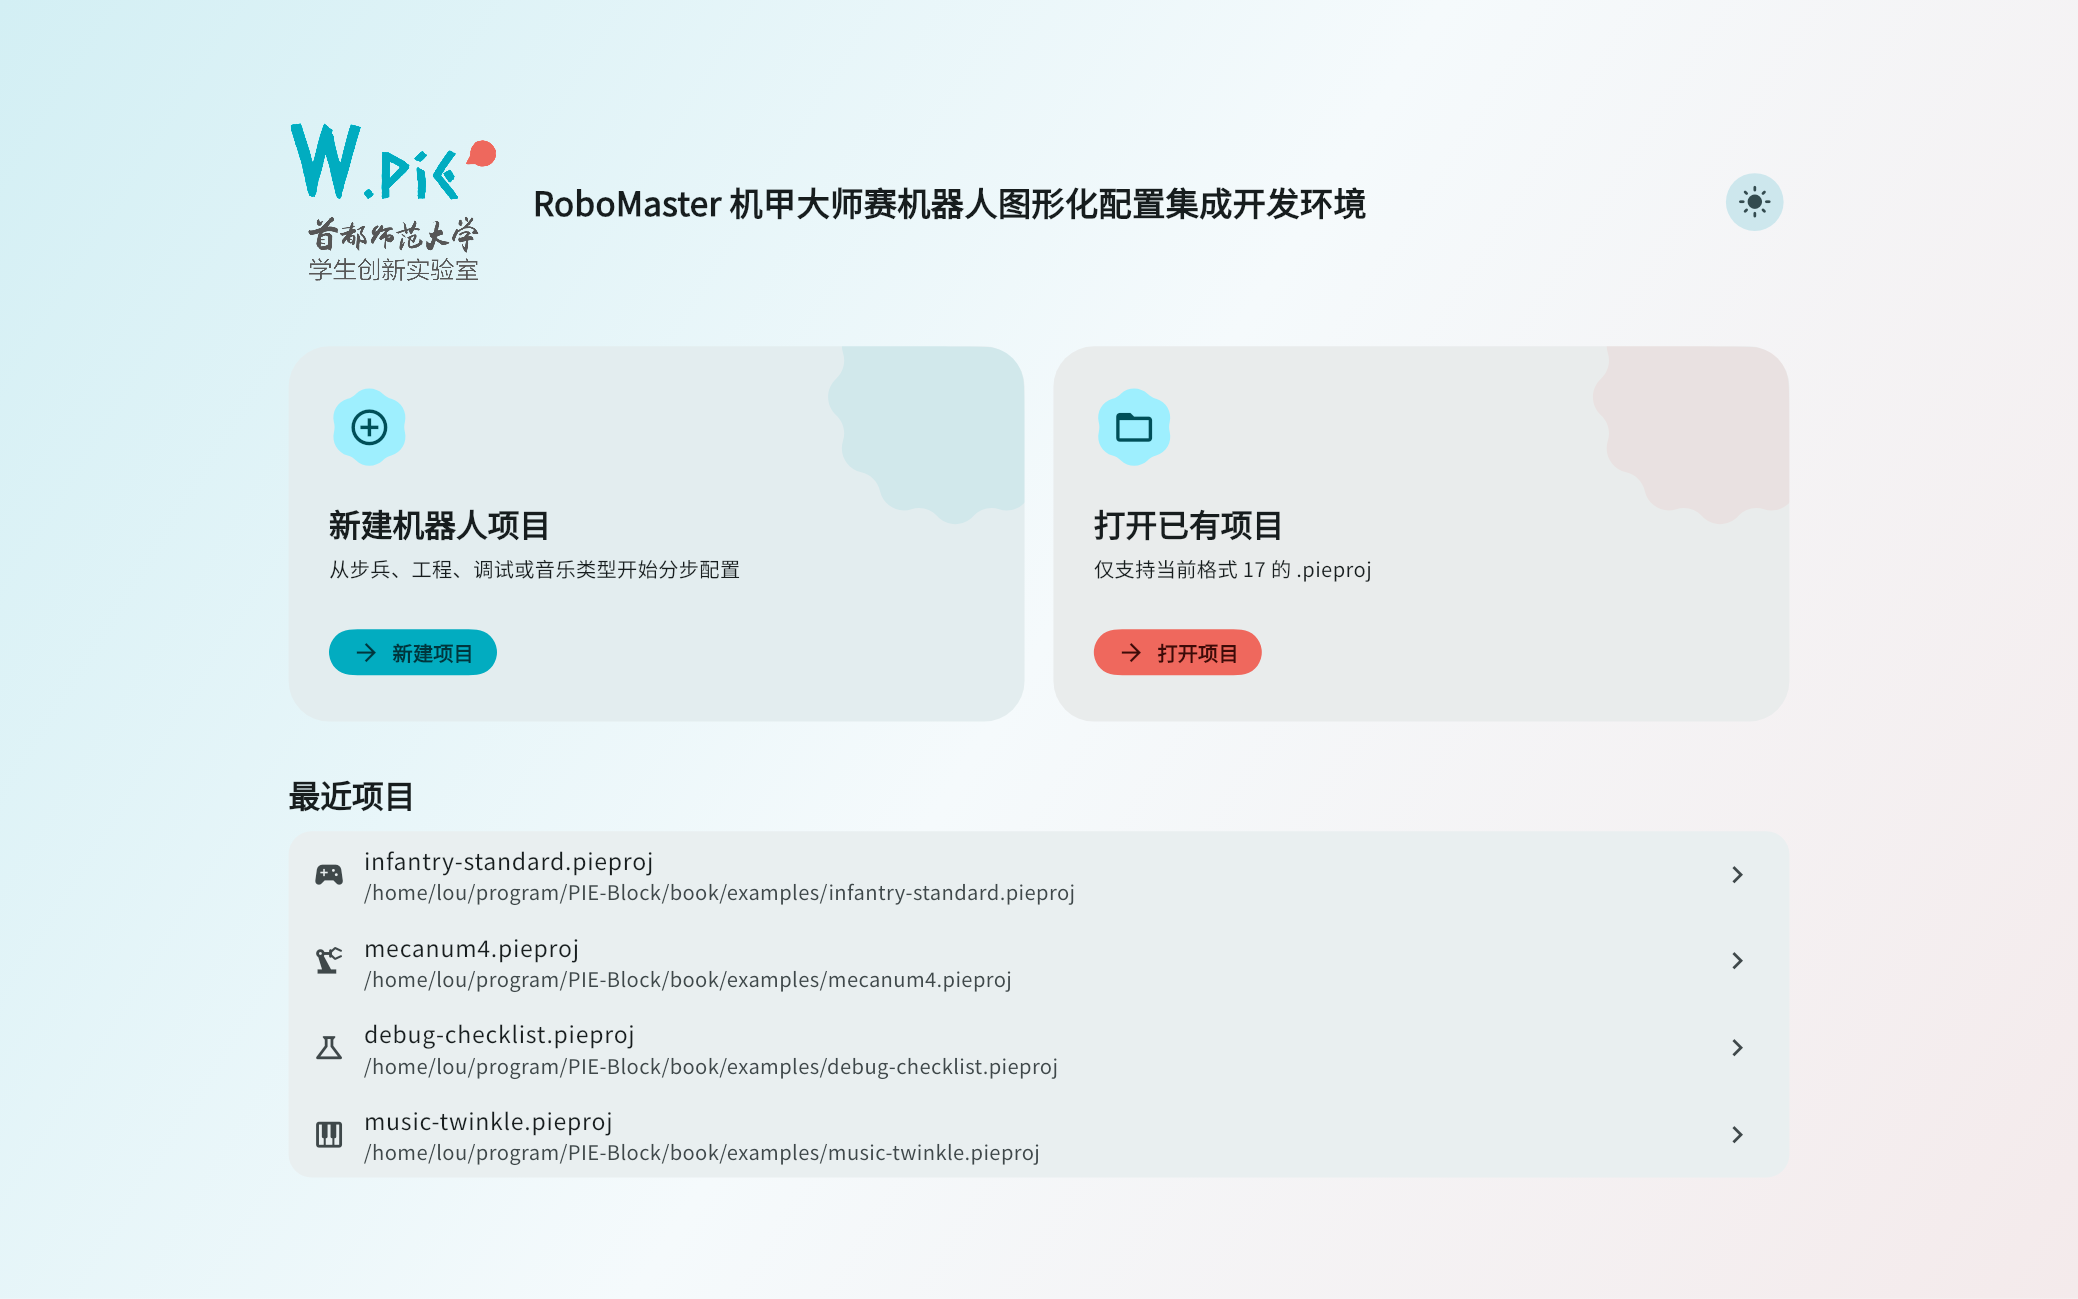
\includegraphics[width=0.95\linewidth]{image/ch10/10-1-home-recent.png}
  \caption{首页与“最近项目”：新建/打开两个入口，下方按类型图标列出
  最近打开的工程}
  \label{fig:ch10-home}
\end{figure}

\section{排障路径}

PIE-Block 的故障可以按“配置 $\rightarrow$ 代码 $\rightarrow$ 烧录”三级
定位，与软件的分步结构一致：

\begin{enumerate}
  \item \textbf{配置层}：检查页有错误/警告，逐条点击跳回修改。方向类
        问题（车不动、方向反）查第~\ref{ch:chassis}~章的速查表；
  \item \textbf{代码层}：公式类问题用“试算表达式”核对典型输入，表达式
        编译检查确认整个固件能编译（第~\ref{ch:gencheck}~章）；
  \item \textbf{烧录层}：看“进度与日志”——检测不到设备、写块无响应、
        部署失败，各有明确提示（第~\ref{ch:linkdebug}~章与附录~B）。
\end{enumerate}

各级都通过后仍异常的，问题多半在硬件：供电、接线、通道、机械干涉。软件
已经把“纸面错误”挡在了烧录之前，实车调试只剩下真实的物理问题——这
正是“先检查再生成”的设计意图。

\section{Web、Android 与桌面端的差异}

PIE-Block 有桌面（Windows/Linux）、Web 与 Android 三种形态，核心的
配置、检查与代码生成在所有平台一致，差异集中在需要本机能力的部分：

\begin{center}
\begin{tabular}{@{}lll@{}}
\toprule
能力 & 桌面端 & Web / Android \\
\midrule
配置、检查与摘要 & 全部可用 & 全部可用 \\
生成代码、C 代码导出 & 可用 & 可用 \\
表达式解析校验 & 可用 & 可用 \\
表达式编译检查（SDCC） & 可用 & Web 不可用；Android 用内置原生库 \\
汇编列表对照 & 可用 & Web 不可用；Android 可用 \\
USB-HID 烧录 & 可用 & Web 不可用；Android 经 OTG 可用 \\
Keil C251 构建与许可证 & 可用 & 不可用 \\
\bottomrule
\end{tabular}
\end{center}

简单说：Web 版适合“改配置、写表达式、看生成代码”；编译与烧录回到
桌面端（或 Android 的 OTG 直连）完成。

\section{进阶的三条路}

\begin{itemize}
  \item \textbf{研究产物}：从 \texttt{main.rst} 读 C 与 251 指令的对照
        （第~\ref{ch:linkdebug}~章），从 \texttt{main.c} 读固件结构——
        混控、武器逻辑与提示音都在里面，是学习 STC32G 开发的入口；
  \item \textbf{命令行与自动化}：代码生成器提供 CLI 接入（把配置直接
        编译成 C 与固件产物），可以接入 CI 或脚本化流程；生成的固件
        也可以用独立 Keil 工程构建；
  \item \textbf{二次开发}：PIE-Block 本身开源（Flutter 桌面/Web/Android
        与多个 Dart 包），校验器、代码生成器与工具链封装都有清晰的模块
        边界，适合在课程设计或实验室工具链改造中复用。
\end{itemize}

全书正文到此结束。附录 A 汇总硬件接口与引脚速查，附录 B 收录高频问题，
附录 C 是术语表——排查与复习时翻回来用。
